\documentclass[a4paper]{scrreprt}
 
\usepackage[german]{babel}
\usepackage[utf8]{inputenc}
\usepackage[T1]{fontenc}
\usepackage{ae}
\usepackage[bookmarks,bookmarksnumbered]{hyperref}
\usepackage{graphicx}
\graphicspath{ {Images/} }
\setcounter{secnumdepth}{5}
 
\begin{document}
 
    \begin{flushright}
        
\includegraphics[scale = 0.7]{kit-logo.jpg}\\[0.5cm]
        % 
\includegraphics[scale = 1]{teco.jpg}
    \end{flushright}
    % 
\includegraphics[scale = 0.5]{kit-logo.jpg} \hspace{4cm} 
\includegraphics[scale = 1]{teco.jpg}
    \vspace*{2cm} 

    \begin{center} \large 
    
        Praxis der Softwareentwicklung
        \vspace * {1.5cm}

<<<<<<< HEAD
        {\textbf \huge Mind Rate}
		
        \vspace*{1cm}
		
        {\textbf \large Ein interaktives Werkzeug f\"ur Studie nach Experience-Sampling-Method (ESM)}
=======
        \textbf{\huge Mind Rate}
		
        \vspace*{1cm}
		
        \textbf{\large Ein interaktives Werkzeug f\"ur Studie nach Experience-Sampling-Method (ESM)}
>>>>>>> origin/master
        \vspace*{1cm}

        {\large Pflichtenheft}
        \vspace*{2cm}

        Shanshan Du, Yi Ge, Renhan Lou, Ruoheng Ma, Haobin Tan
        \vspace*{1cm}

        02. Dezember 2016
        \vspace*{2.5cm}


        Betreuung: Anja Exler, Erik Psescara\\[1cm]
        Technology f\"ur Pervasive Computing\\[0.5cm]
        Karlsruher Institut für Technologie
    \end{center}
 
    % Die abstract-Umgebung kann bei Bedarf aus dem Pflichtenheft entfernt werden
    % \begin{abstract}
    %     Dies ist ein beispielhaftes Pflichtenheft in \LaTeX. Das Pflichtenheft
    %     beschreibt in konkreter Form, wie der Auftragnehmer die Anforderungen des
    %     Auftraggebers zu lösen gedenkt - das sogenannte wie und womit. Der Auftraggeber
    %     beschreibt vorher im Lastenheft möglichst präzise die Gesamtheit der
    %     Forderungen - was er entwickelt oder produziert haben möchte. Erst wenn der
    %     Auftraggeber das Pflichtenheft akzeptiert, sollte die eigentliche Arbeit beim
    %     Auftragnehmer beginnen.
    %     \vspace{1cm}
 
    %     Quelle: \url{http://de.wikipedia.org/wiki/Pflichtenheft} und Lehrbuch der
    %     Objektmodellierung von Heide Balzert
    %     \vspace{0.5cm}
 
    %     Quellcode: \url{http://www.karllorey.de/informatik-studium/vorlesungen/softwarepraktikum/pflichtenheft-in-latex/}
    % \end{abstract}
 
    % Platzierung des Inhaltsverzeichnisses
    \tableofcontents
    
    % \chapter{Einleitung}
    %     {\bf \large Experience sampling method\footnote{\url{https://en.wikipedia.org/wiki/Experience_sampling_method}} (ESM)}\\
        
    %     The experience sampling method, also referred to as a daily diary method, or ecological momentary assessment (EMA), is a research methodology that asks participants to stop at certain times and make notes of their experience in real time. The point is for them to record temporal things like feelings while in the moment (right then, not later; right there, not elsewhere). They can be given a journal with many identical pages. Each page can have a psychometric scale, open-ended questions, or anything else used to assess their condition in that place and time. Online ESM studies can also operate fully automatized.\footnote{van der Krieke; et al. (2015). ``HowNutsAreTheDutch (HoeGekIsNL): A crowdsourcing study of mental symptoms and strengths". International Journal of Methods in Psychiatric Research. 25 (2): 123–144. doi:10.1002/mpr.1495. PMID 26395198} The experience sampling method was developed by Larson and Csikszentmihalyi.\footnote{Larson, R., \& Csikszentmihalyi, M. (1983). ``The experience sampling method". New Directions for Methodology of Social and Behavioral Science, 15, 41-56.} \\

    %     There are different ways to signal participants when to take notes in their journal or fill-out a questionnaire,\footnote{Hektner, J.M., Schmidt, J.A., Csikszentmihalyi, M. (Eds.). (2006). Experience Sampling Method: Measuring the Quality of Everyday Life. Sage Publications, Inc. ISBN 978-1-4129-2557-0} like using preprogrammed stopwatches. An observer can have an identically programmed stopwatch, so the observer can record specific events as the participants are recording their feelings or other behaviors. It is best to avoid letting subjects know in advance when they will record their feelings, so they can't anticipate the event, and will just be ``acting naturally" when they stop and take notes on their current condition. Conversely, some statistical techniques require roughly equidistant time intervals, which has the limitation that assessments can be anticipated. Validity in these studies comes from repetition, so you can look for patterns, like participants reporting greater happiness right after meals. These correlations can then be tested by other means for cause and effect, such as vector autoregression,\footnote{"Temporal Dynamics of Health and Well-Being: A Crowdsourcing Approach to Momentary Assessments and Automated Generation of Personalized Feedback (2016)". Psychosomatic Medicine. doi:10.1097/PSY.0000000000000378} since ESM just shows correlation.

 
    \chapter{Zielbestimmung}
    % Dieses Kapitel dient der Bestimmung von Zielen und nicht für deren Verwendung
    % notwendige Funktionen.
        Die Firma soll durch das Produkt in die Lage versetzt werden, psychologische Studien nach Experience-Sampling-Method (ESM) durchzuf\"uhren und Feedbacks der Studien zu erhalten.\\

        \noindent Das Produkt besteht aus zwei Teilsysteme, Web Server f\"ur den Versuchsleiter und Android Anwendung f\"ur die Probanden.
 
 
        \section{Musskriterien}
            % Musskriterien: Für das Produkt unabdingbare Leistungen, die in jedem Fall
            % erfüllt werden müssen \footnote{gezwungen sein, etwas zu tun (Dies ist eine
            % beispielhafte Fußnote).}. Das System ist ohne diese Funktionen für seinen
            % gedachten Zweck nicht einsetzbar.
            \vspace*{0.3cm}

            \subsection{Web-server f\"ur Versuchsleiter}
                \vspace*{0.2cm}

                \subsubsection{Verwalten von Teilnehmer der Untersuchung}
                    \begin{itemize}
                        \item Probandsstatus erfassen (z.B. Proband-ID, Alter, Geschlecht, Beruf)
                        \item Anmelden f\"ur Durchf\"uhrung der Untersuchung
                    \end{itemize}
            
                \subsubsection{Verwalten der Frageb\"ogen}
                    \begin{itemize}
                        \item Ausw\"ahlen von Prob\"ande nach verschiedenen Kriterien vor Erstellung der Frageb\"ogen
                        \item Erstellen, \"Andern von Untersuchungsfragen f\"ur unterschiedliche Probandsgruppe
                        \item Erstellen, \"Andern von Scale und Optionen der Antworten
                        \item Setzen, \"Andern von G\"ultigkeitszeitbereich der Untersuchungsfragen
                        \item Setzen, \"Andern von H\"aufigkeit der Notifikationen zur Antworten
                        % \item Senden von Feedback und Motivation zu Probanden
                    \end{itemize}

                \subsubsection{Erfassen von Ergebnisse der Untersuchung}
                    \begin{itemize}
                        \item Exportieren von Daten  
                    \end{itemize}
            \vspace*{2cm}

            \subsection{Android Anwendung f\"ur Probanden}
                \vspace*{0.2cm}

                \subsubsection{Anmelden f\"ur Beteiligung der Studie}
                
                \subsubsection{Antwort auf Untersuchungsfragen}
                    \begin{itemize}
                        \item regelm\"assige Notifikation zur Antworten
                        \item Untersuchungsfragen beantworten
                    \end{itemize}
                
                \subsubsection{Verwalten von Antworten}
                    \begin{itemize}
                        \item lokales Speichern von Antworten
                        \item Protokollieren von Zeitpunkt der Antwort
                        \item Hochladen von Antworten auf den Server
                    \end{itemize}

                \subsubsection{Zurgreifen einiger Sensoren von Handy}
                    \begin{itemize}
                        \item Zugreifen von Temperatursensor
                        \item Zugreifen von GPS
                    \end{itemize}
                \vspace*{0.5cm}

 
        \section{Wunschkriterien}
            \vspace*{0.3cm}
            % Kannkriterien: Die Erfüllung der Kannkriterien ist erwünscht, jedoch nicht
            % unbedingt notwendig. Sie sollten nur angestrebt werden, falls noch ausreichend
            % Kapazitäten vorhanden sind.
            
            \subsection{Web-server f\"ur Versuchsleiter}
                \begin{itemize}
                     % \item Emailbest\"atigugn beim (erfolgreichen) Anmelden
                    \item Erm\"oglichen von ``angemeldet bleiben"
                    \item Erzeugen von verschiedenen (Statistik-)Diagramme f\"ur hochgeladene Daten (z.B. S\"aulendiagramm, Kreisdiagramm) 
                    \item Unterst\"utzen von unterschiedlichen Sprachen
                    
                \end{itemize}

            \subsection{Android Anwendung f\"ur Probanden}
                \begin{itemize}
                    \item Erm\"oglichen von ``angemeldet bleiben"
                    \item Unterst\"utzen von unterschiedlichen Sprachen
                    \item Wechseln von Theme der Anwendung
                \end{itemize}
                \vspace*{0.5cm}

 
        \section{Abgrenzungskriterien}
            % Abgrenzungskriterien: Diese Kriterien sollen bewusst nicht erreicht werden.
            \begin{itemize}
                \item Keine verteilte Datenbank, keine Echtzeitanforderungen, keine synchronisierten Datenbankzugriffe
                \item Keine Unterst\"utzung f\"ur iOS
            \end{itemize}
 
    \chapter{Produkteinsatz}
        Das Produkt dient zur Sammlung der Versuchsdaten aus psychologischen Versuchen nach ESM. Damit bietet sie für Versuchsleiter eine Lösung, ESM-Versuchen durchzuführen. Diese Tätigkeit soll zusätzlich im Internet und auf dem Smartphone möglich sein.
 
        \section{Anwendungsbereiche}
            \begin{itemize}
                \item Akademischer / Sozialwissenschaftlicher Anwendungsbereich
                \item Statistischer Anwendungsbereich
            \end{itemize}
 
        \section{Zielgruppen}
            \begin{itemize}
                \item Versuchsleiter eines ESM-Versuchs
                \item Teilnehmer des Versuchs
            \end{itemize}
 
        \section{Betriebsbedingungen}
            \begin{itemize}
                \item Versuchsleiter: Büroumgebung
                \item Versuchsteilnehmer: im alltäglichen Leben aufs Smartphone
                \item Betriebszeit rund um die Uhr, läuft unbeaufsichtigt
            \end{itemize}
 
    \chapter{Produktumgebung}
        Eine Client-Server Architektur mit 2 Client-Typen: der Web-Client für Versuchsleiter und der Smartphone-Client für Versuchsteilnehmer

        \section{Software}
            \begin{itemize}
                \item Serverseite
                    \begin{itemize}
                        \item  Läuft auf Linux
                        \item Alle Softwares der Serverseite werden durch Docker verpackt
                        \item Datenbank: SQLite, verwaltet durch das Django-Framework
                        \item Programmiersprache: Python 3
                        \item Web server: Nginx
                    \end{itemize}
                \item Clientseite
                    \begin{itemize}
                        \item Web-Client\\
                             Web-Browser, Referenzstandard Google Chrome 54
                        \item  Smartphone-Client\\
                             Android, Referenzstandard Android 7.1 Nougat
                    \end{itemize}
            \end{itemize}
 
        \section{Hardware}
            \begin{itemize}
                \item Serverseite\\
                    Leistungsstarke Standardrechner
                \item  Web-Client\\
                    Standardrechner
                \item Smartphone-Client\\
                    Standardsmartphone
            \end{itemize}

    \chapter{Funktionale Anforderungen}

		\section{Web}
	        \begin{itemize}
	            \item \textbf{/F10/Anmelden oder Registrieren der Leiter}
		          
	            	\par \textbf{Ziel: }Registrieren oder Anmelden der Versuchsleiter in der Web-Verwaltungssystem
	            	\par \textbf{Vorbedingung (Registrieren): }-keine-
	            	\par \textbf{Vorbedingung (Anmelden): }Ein Konto des Leiters soll vorhanden sein.
	            	\par \textbf{Nachbedingung (erfolgreiches Registrieren): }Der Leiter bekommt eine Bestätigungsmail und kann sich mit dem neu erzeugten Konto anmelden.
	            	\par \textbf{Nachbedingung (erfolgreiches Anmelden): }Der Leiter ist in der Verwaltungssystem angemeldet und kann seine Versuche verwalten.
	            	\par \textbf{Nachbedingung (Fehlschlag): }Der Leiter bleibt unangemeldet.
	            	\par \textbf{Akteure: }Versuchsleiter
	            	\par \textbf{Auslösendes Ereignis: }Der Leiter vesucht erneut sich zu registrieren oder anzumelden.
	            	\par \textbf{Beschreibung: }
		            	\begin{enumerate}
		            		\item Beim Registrieren soll der Leiter eine gültige Email-Adresse und ein gültiges Passwort eintragen. Diese Daten werden von dem Datenbank gespeichert und der Server erzeugt ein neues Konto. Danach empfängt der Leiter eine Bestätigungsmail und kann sich mit dem neuen Konto anmelden.
			            	\item Beim Anmelden soll der Leiter die registrierte Email-Adresse und sein Passwort eingeben. Wenn die Email-Adresse und das Passwort stimmen überein, dann wird der Leiter in die Verwaltungsseite weitergeleitet.
		            	\end{enumerate}
	            	\par \textbf{Erweiterung: }
	            	\par \textbf{Alternativen: }
	            	
	            \item /F20/Vergessenes Passwort neu zu setzen
	            	\par Wenn ein Leiter sein Passwort vergessen hat, kann er auf “Passwort Vergessen” klicken und in der weitergeleiteten Seite seine Email-Adresse eingeben. Danach empfängt er ein Bestätigungsemail mit einem Link. Durch dieses Link ist er in die “Passwort neu setzen” Seite weitergeleitet und sein neues Passwort wird in dem Datenbank gespeichert.

	            \item /F30/Erstellung eines Fragebogens (Inhalt, regelmäßige Sendungszeit, Zeitzone, gültiger Zeitraum für die Antworten)
	            	\par Nach der Anmeldung ist der Leiter in die Verwaltungsseite geleitet. Da kann er Fragebogen erstellen und die Sendungszeit festlegen. Es gibt dabei noch eine Zeitzone-Option. Mit dieser Option kann der Leiter sich entscheiden, ob das Fragebogen abgesehen von Zeitzonen um dieselbe Uhrzeit geschickt wird oder um dieselbe Zeit je nach den Zeitzonen. Außerdem kann der Leiter festlegen, wie lange ist der Zeitraum für eine gültige Antwort.
	            	
	            \item /F40/Dashboard
	            	\par 
	            	
	            \item /F50/Exportieren von Daten
		         	\par Der Leiter kann alle Antworten und die Metadata (z.B. Anzahl von Teilnehmer, Verhältnis zwischen positiven und negativen Antworten) hinsichtlich seiner allen Fragebogen in Form von CSV exportieren.

			\end{itemize}
    
		    \section{App}
        
        \begin{itemize}
            \item \textbf{/F70/Anmelden der Probanden}
            
				\par \textbf{Ziel: }Anmelden der Probanden in der App und Sammeln der Versuchsteilnehmerdaten während erstem Anmelden
				\par \textbf{Vorbedingung: }-keine-
				\par \textbf{Nachbedingung (erstes Anmelden): }Versuchsteilnehmerdaten liegen vor und Proband ist angemeldet
				\par \textbf{Nachbedingung (kein erstes Anmelden): }Proband ist angemeldet
				\par \textbf{Akteure: }Proband
				\par \textbf{Auslösendes Ereignis: }Proband öffnet die App
				\par \textbf{Beschreibung: }
				\par 1. Wenn der Proband zum ersten Mal die App öffnet: Der Proband meldet sich mit der ID des Versuchs an und gibt die 
				 von Versuchsleiter angeforderten Versuchsteilnehmerdaten ein. Eine einzigartige, mit dem Handy verbundene Proband-ID wird generiert und dem Proband zugeteilt. Die Proband-ID wird nicht gezeigt aber in der App gespeichert. Die App wechselt dann auf die Hauptseite.
				\par 2. Wenn der Proband sich mindestens einmal angemeldet hat: Die App wechselt automatisch auf die Hauptseite.
				\par \textbf{Alternativen: }
								

            \item \textbf{/F80/Antworten eines Fragebogens}

            	\par \textbf{Ziel: }Sammeln der Antworten auf den Fragebogen
            	\par \textbf{Vorbedingung: }Anmeldung und mindestens ein vorliegender Fragebogen in der App
            	\par \textbf{Nachbedingung: }die Antworten werden lokal gespeichert
            	\par \textbf{Akteure: }Proband
            	\par \textbf{Auslösendes Ereignis: }Proband meldet sich an
            	\par \textbf{Beschreibung: }
            	\par 1. Wenn der Versuchsleiter einen Fragebogen sendet, schickt die App eine Notifikation.
            	\par 2. Nachdem der Proband sich angemeldet hat, liegt die App auf der Hauptseite mit einer Liste der auszufüllenden Fragebögen. Der Proband wählt einen Fragebogen aus und beantwortet alle darauf stehenden Fragen. Im Anschluss klickt der Proband auf "Senden" und die Antworten werden lokal gespeichert.
            	\par \textbf{Alternativen: }
            	

            \item \textbf{/F90/Versenden der Antworten eines Fragebogens}
            
            \par \textbf{Ziel: }Versenden der Antworten an den Server
            \par \textbf{Vorbedingung: }die Antworten werden lokal gespeichert
            \par \textbf{Nachbedingung (Erfolg): }die Antworten werden auf dem Server gespeichert
            \par \textbf{Nachbedingung (Fehlschlag): }die Antworten werden nicht auf dem Server gespeichert
            \par \textbf{Akteure: }App und Server
            \par \textbf{Auslösendes Ereignis: }die Netzwerkverbindung ist verfügbar und es gibt lokal gespeicherte Antworten
            \par \textbf{Beschreibung: }
            \par Wenn die Netzwerkverbindung vorhanden ist, schickt die App die verfügbaren Antworten an den Server und die Antworten werden auf dem Server gespeichert. 
            \par \textbf{Alternativen: }

        \end{itemize}
 
    \chapter{Produktdaten}
        \section{Versuchsleiterdaten}
            \begin{itemize}
                \item /D10/ Über einen Versuchsleiter sind folgende Daten zu speichern:
                    \par Name (Anrede, Titel, Vorname, Nachname), Mailadresse (als Kontonummer im System)
                    
                \item /D20/ Macht ein Versuchsleiter Versuche, dann sind folgende Daten zu speichern:
                    \par Versuchsummern der zum Versuchsleiter gehörten Versuchen
            \end{itemize}
            
        \section{Versuchsteilnehmerdaten}
            \begin{itemize}
                \item /D30/ Über einen Versuchsteilnehmer sind folgende Daten zu speichern:
                    \par Name (Anrede, Titel, Vorname, Nachname), Mailadresse (als Kontonummer im System), Telefonnummer, demographische Daten (Geburtsdatum, Beruf, Geschlecht), Notiz
                
                \item /D40/ Nimmt ein Versuchsteilnehmer an Versuchen teil, dann sind folgende Daten zu speichern:
                    \par Versuchsnummern der daran beteiligten Versuchen
            \end{itemize}
            
        \section{Versuchsdaten}
            \begin{itemize}
                \item /D50/ Über einen Versuch sind folgende Daten zu speichern:
                    \par Versuchsnummer, Versuchsname, Anfangs- und Endedatum, Mailadresse der Versuchsleiter, Notiz
                    
                \item /D60/ Hat ein Versuch Teilnehmer, dann sind folgende Daten zu speichern:
                    \par Mailadressen der Versuchsteilnehmer
                    
                \item /D70/ Hat ein Versuch Fragen, dann sind folgende Daten zu speichern:
                    \par Fragenummer der Fragen
            \end{itemize}
            
        \section{Fragendaten}
            \begin{itemize}
                \item /D80/ Über eine Versuchsfrage sind folgende Daten zu speichern:
                    \par Fragenummer, Fragetyp, Inhalt der Frage, Versuchsnummer des zugehörigen Versuchs
                    
                \item /D90/ Wird eine Frage im Versuch erscheinen, dann sind folgende Daten zu speichern:
                    \par Erscheinungskriterium, Abgabetermin
                    
                \item /D100/ Wird eine Frage von Versuchsteilnehmern beantwortet, dann sind folgende Daten zu speichern:
                    \par Mailadressen der Antwortgeber, Abgabezeit der Antworten, Inhalt der Antworten
            \end{itemize}
 
   \chapter{Nichtfunktionale Anforderungen}
        \begin{itemize}
            \item /NF10/Reaktionszeit

            	\par Die App darf nicht mehr als \_ Sekunden Reaktionszeit haben und die Ladezeit muss unter \_ Sekunden liegen.

                
        \end{itemize}
 
        \begin{itemize}
            \item /NF20/Registrierung

            	\par Die Registrierung erfolgt unter Angabe einer E-Mail Adresse und einem Passwort.
                
        \end{itemize}
        \begin{itemize}
            \item /NF30/Passwort

            	\par Passwörter müssen mindestens 6-stellig sein. Die App kann angemeldet bleiben.

                
        \end{itemize}
        \begin{itemize}
            \item /NF40/Globalisierung

            	\par Die App ist auf Deutsch und Englisch verfügbar.

                
        \end{itemize}
        \begin{itemize}
            \item /NF50/Daten speichern

            	\par Die Antworten jedes Fragebogens von den Probanden muss ins Handy gespeichert werden.

                
        \end{itemize}
        \begin{itemize}
            \item /NF60/Größe der App

            	\par Die App darf nicht mehr als \_ Mb auf dem Handy benötigen.


                
        \end{itemize}
        \begin{itemize}
            \item /NF70/Integration ins Google Play Store

            	\par Die App soll ins Google Play Store integriert werden.


                
        \end{itemize}
 
    \chapter{Benutzungsoberfläche}
    %     Benutzungsoberfläche: grundlegende Anforderungen, Zugriffsrechte
 
        \begin{figure}[ht]
            \centering
            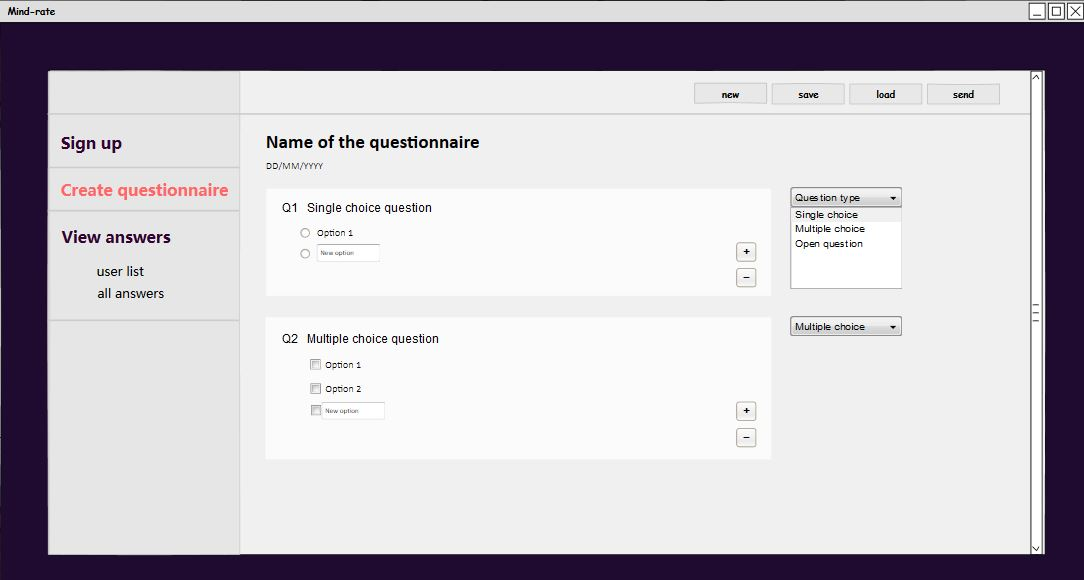
\includegraphics[scale = 0.4]{web.jpg}
            \caption{GUI Entwurf - Web interface}
        \end{figure}
	
	\begin{figure}[ht]
            \centering
            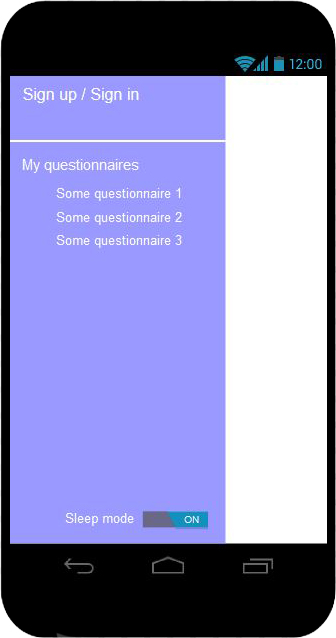
\includegraphics[scale = 0.3]{android1.jpg}
            \caption{GUI Entwurf - Android App [1]}
        \end{figure}
	
	\begin{figure}[ht]
            \centering
            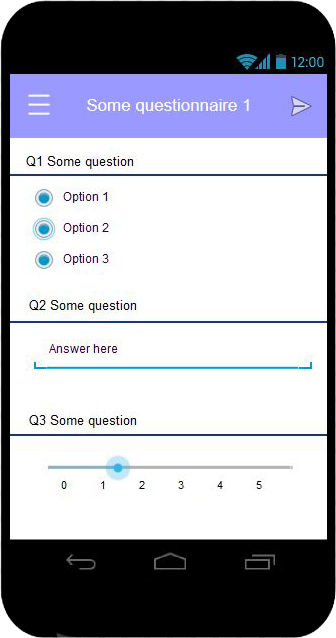
\includegraphics[scale = 0.3]{android2.jpg}
            \caption{GUI Entwurf - Android App [2]}
        \end{figure}

    \chapter{Globale Testfälle}

    \chapter{Systemmodelle}

        \section{Szenarien}

        \section{Anwendungsf\"alle}

            \newpage
            \subsection{Anwendungsfalldiagramm} 
                \vspace{0.4cm}
                \begin{center}
                    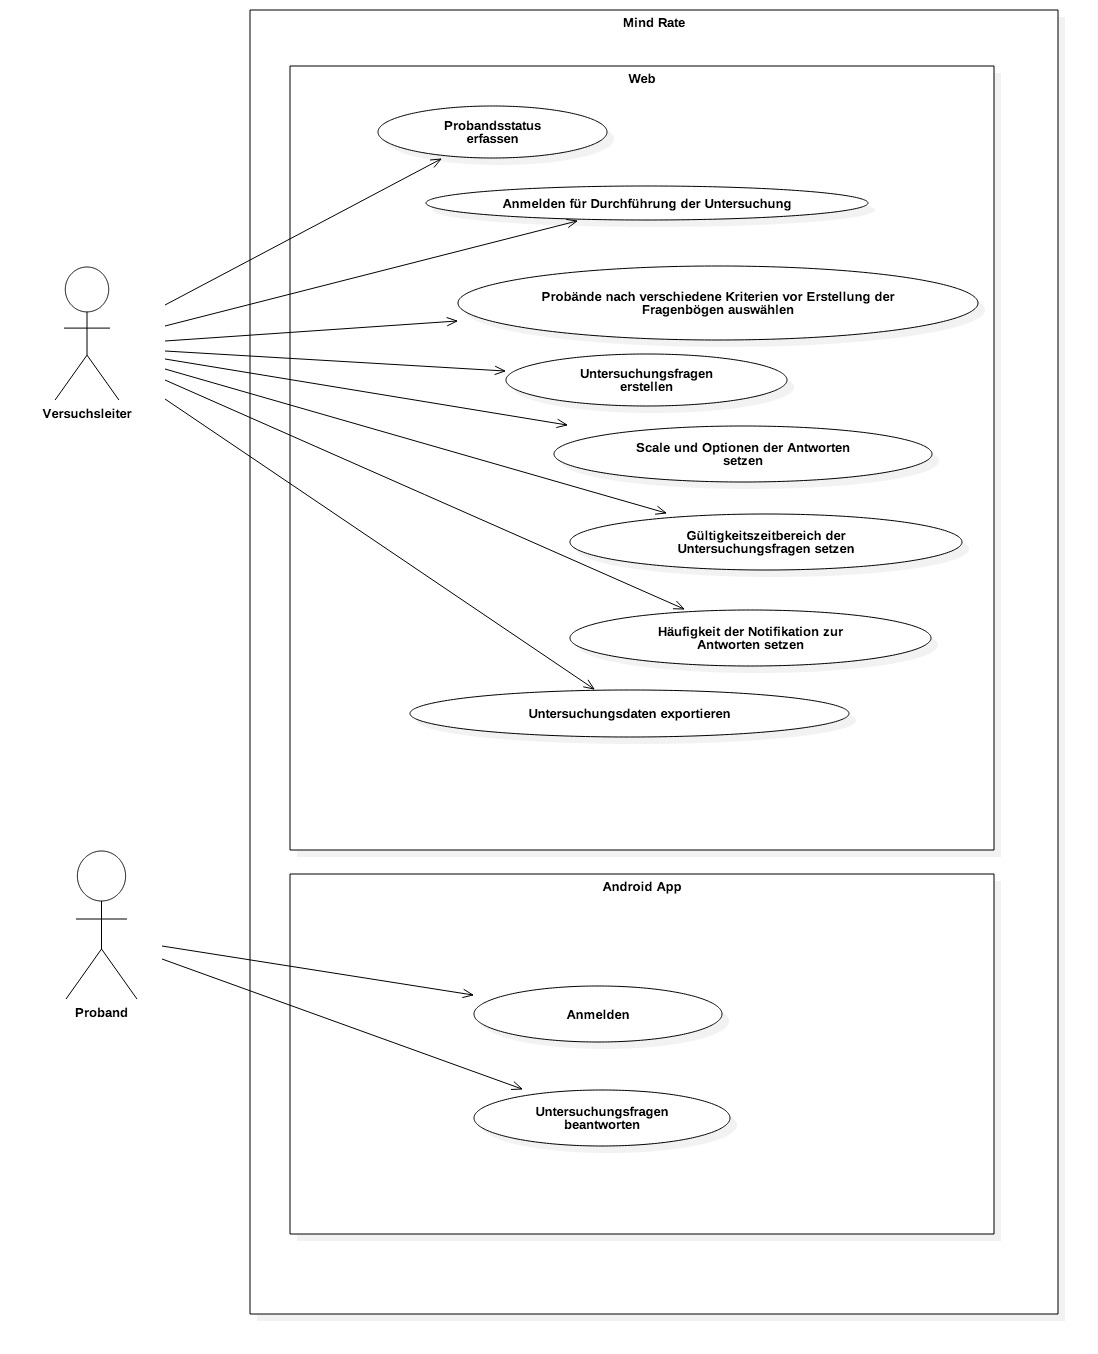
\includegraphics[scale = 0.4]{UseCaseDiagram1.jpg}
                \end{center}

        \newpage
 
    \chapter{Qualitätsziele}
        Qualiätsziele: Allgemeine Ziele sind meistens Änderbarkeit und Wartbarkeit.
        Ziele sollten jedoch grundsätzlich messbar, spezifisch und relevant sein.
 
    \chapter{Glossar}
 
    % Abbildungsverzeichnis
    \listoffigures
 
\end{document}
